\documentclass{article}

% if you need to pass options to natbib, use, e.g.:
% \PassOptionsToPackage{numbers, compress}{natbib}
% before loading nips_2016
%
% to avoid loading the natbib package, add option nonatbib:
% \usepackage[nonatbib]{nips_2016}

\PassOptionsToPackage{numbers,sort&compress}{natbib}
\usepackage[final]{nips_2016} % produce camera-ready copy

\usepackage[utf8]{inputenc} % allow utf-8 input
\usepackage[T1]{fontenc}    % use 8-bit T1 fonts
\usepackage{hyperref}       % hyperlinks
\usepackage{url}            % simple URL typesetting
\usepackage{booktabs}       % professional-quality tables
\usepackage{amsfonts}       % blackboard math symbols
\usepackage{nicefrac}       % compact symbols for 1/2, etc.
\usepackage{microtype}      % microtypography
\usepackage{graphicx}

\usepackage{multirow}
\usepackage{subcaption}
\usepackage{float}
\title{Assessing ML Models for Species Data Modelling}  

% The \author macro works with any number of authors. There are two
% commands used to separate the names and addresses of multiple
% authors: \And and \AND.
%
% Using \And between authors leaves it to LaTeX to determine where to
% break the lines. Using \AND forces a line break at that point. So,
% if LaTeX puts 3 of 4 authors names on the first line, and the last
% on the second line, try using \AND instead of \And before the third
% author name.

\author{
  YU-CHI CHU\\
\\
}

\begin{document}

\maketitle

\begin{abstract}

 The study compares the performance of machine learning models and different data preparation techniques for predicting sightings using species data from iNaturalist and world climatic variables from WorldClim. Our aim is to produce a model that cane be generalised and does not have to be tuned and trained for each species prediction.  After preprocessing, Random Forest and XGBoost performed best, with Random Forest achieving 0.786 PR AUC. MaxEnt was also found to be effective but not efficient due to its high computational demand. Overall, Random Forest with Principal Component Analysis (PCA) offered the best balance of efficiency and a high evaluation score.  
\end{abstract}

% \section{Instructions}

% \textit{The \textit{report} should use this template and be 6 pages in length. Do not change the fontsize or layout. It should be compilable with pdflatex.}

% \textit{Structuring the text as follows is recommended, but not mandatory.}

\section{Introduction}

The aim of this work is to compare the performance of different machine learning (ML) models and pre-processing steps in predicting the sightings of a species at a location.   We use data on the sightings of the species, the sightings of other species plus climate and elevation data.  

The complex relationships between species and their environment, and the big increase in data available from sources such as remote sensing and citizen scientists have driven interest in ML for species data modelling (SDM)\cite{sdm} over the last 20 years.  The data used in SDM falls into two main categories: Presence Only and Presence-Absence data\cite{sdm} (Beery et al, 2021).  The former, which includes the data collected from iNaturalist\cite{iNaturalist} used in our analysis, is Presence Only and is based on observations of a species at a location.  It does not specifically say the species is absent at a location but rather a sighting has not been recorded.   Challenges with such data include training a model without definitive information on where the species is absent\cite{presence_only} (Hastie and Fithian, 2013) and sighting locations being heavily biased to areas accessible to observers\cite{sampling-bias} (Reddy and Davalos. 2003). 

A range of different ML models have been used for SDM.  The non-linear relationships given the complexity of ecosystems,  imbalanced and correlated data, non i.i.d data, the need for transparency on the most important features and the afore mentioned presence only data have all impacted choices.   Decision Tree structures able to cope with the non-linear, non-i.i.d and imbalanced data have been used by multiple authors including Random Forests\cite{rf} (Cutler et al., 2007) and XGBoost\cite{xgboost} (Elith et al, 2008).  SVM has also been used \cite{svm}(Drake et al., 2006).   Pseudo-absence data has been introduced to these models to handle presence only data \cite{presence_only}(Barbet-Massin et al., 2012). The MaxEnt algorithm \cite{MaxEnt} (Phillips et al., 2006 ) was specifically introduced to SDM to cope with presence only data and has been one of the most popular and often cited ML models for datasets of this type.  

A greater understanding of the capabilities of the best ML approaches to predict the location of species is ever more critical given the pressures on biodiversity of climate change and wider human impact.

\section{Data preparation}

The data for our modelling is taken from two sources. The species sighting data is from the train\_extra dataset provided from iNaturalist, and climate and elevation data is from WorldClim\cite{WorldClim}.  The species data consists of 1.3 million sightings of 2,418 species spread across all continents.  We have also used  the 19 bioclimatic variables and elevation data (see appendix) from WorldClim.
\begin{figure}[h]
\centering
\begin{tabular}{ll}
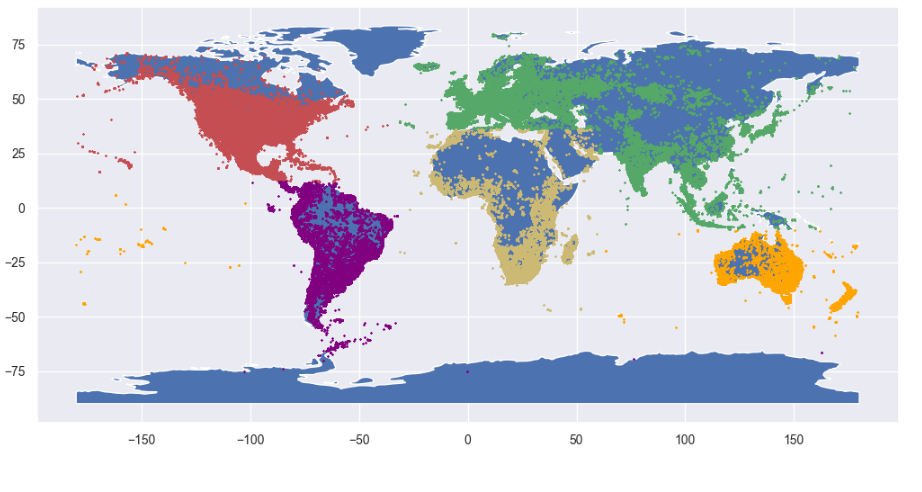
\includegraphics[scale=0.3]{Map_of_sightings.png}&
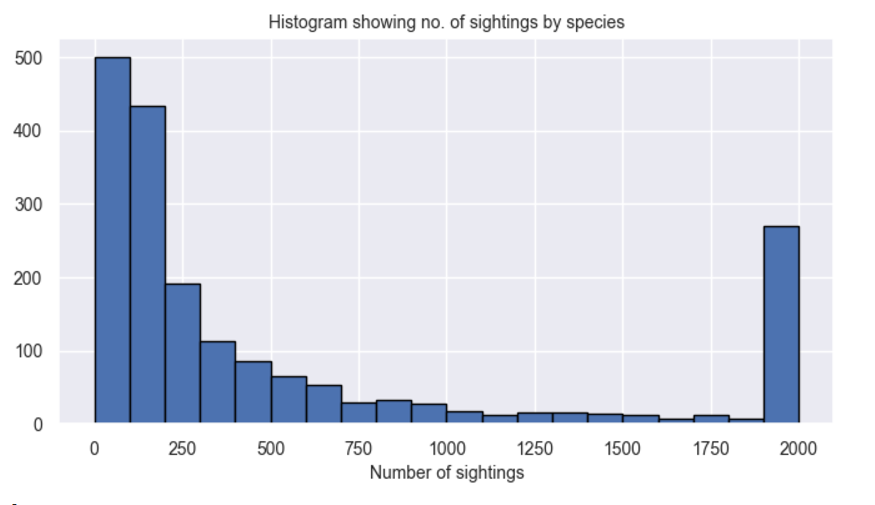
\includegraphics[scale=0.3]{Number of sightings per Species.png}\end{tabular}
\caption{(LHS) Map of sightings by geographic area used in our analysis \\.\hspace{1.3cm}(RHS) Histogram showing the number of sightings for each species}
\label{Fig:Map}
\end{figure}
\begin{table}[h]
    \centering
\begin{tabular}{|c|c|c|c|c|c|l|} \hline 
         Geographic Region&  N America&  S America&  Europe \& Asia&  Africa \& Middle East&  Oceana &Global\\ \hline 
         Species&  684&  537&  773&  705&   387&2418
\\ \hline 
         All sightings&  609841&  109397&  272012&  161534&   186845&1339629
\\\hline
    \end{tabular}
    \caption{Geographic distribution of dataset used in our analysis}
\label{tab:Geographic distribution of dataset}    
\end{table}
The  number of sightings per species in the dataset range from 50 to 2,000.  Whilst the distribution is heavily skewed to the lower sightings per species (Figure 1), over 10\% of the species have 2,000 sightings indicating there are sufficient sightings per individual species to train our ML models. 

We divided the data in to regions for computational efficiency and to reduce the imbalance of sightings verses no sightings.  The splits were informed by analysis of the continuity of species sightings.  It effectively replicated sea boundaries between land masses so we approximated longitude and latitude rectangles for these areas .  

\textbf{Binning Data:} To enable models to run effectively with the computing power available we aggregated data to spatial bins (averaging bioclimate and counting species sightings).  The increased efficiency of a smaller dataset was weighed against the loss of detail from aggregation.  To examine the trade off we used a section of North America (latitudes 15$^{\circ}$- 53$^{\circ}$ \& longitudes -130$^{\circ}$- -60$^{\circ}$).  We assessed bin sizes of 0.25$^{\circ}$, 0.5$^{\circ}$, 1$^{\circ}$ and 2$^{\circ}$. We compared the count of bins with a species present verses all bins in the area (a proxy for the data sparseness) .  We also looked at the distribution of the count of bins for each species to ensure sufficient breadth of geographic sampling to train our ML model.   Our analysis indicates 1$^{\circ}$ bins balance the trade off best with 65\% of possible bins filled and 10\% of the species in the sample area being present in more than 370 bins.   

\subsection{Data Quality: }
To ensure the reliability of our analysis, we first examine the spatial distribution of sightings for each species to identify irregularities.  

\textbf{Convex Hull:} The core of our approach to classifying species as global/local. It constructs a convex polygon encompassing all data points of a species. By analysing its area and perimeter, we can determine the extent of the species' distribution. Table 2 shows a comparison and why we chose this algorithm.
\begin{table}[h]
    \centering    
    \begin{tabular}{|c|c|c|c|} \hline 
 Feature& Convex Hull& DBSCAN& K-Means\\ \hline 
 Data Requirements& Only need 3 data/species& Determine epsilon, minPts&Determine K value\\ \hline 
         Cluster Shape&  Arbitrary shapes&  Arbitrary shapes&  Sphere/Elliptic\\ \hline 
         Complexity&  Efficient&  Expensive&  Sensitive to initialization\\ \hline
    \end{tabular}
\caption{Comparison to different algorithms}
\label{tab:Comparison to different algorithms}  
\end{table}
To further improve the accuracy of our analysis, we employ two outlier detection techniques:

\textbf{LOF}: Applied on local species based on their local density deviation,  suitable for detecting local anomalies and sensitive to parameter selection.

\textbf{Isolation Forest}: Applied on global species, isolating anomalies by partitioning the data space, well-suited for large datasets and global outlier detection.

From the total number of 1339248 data points 61682 were classified as outliers bringing down the number of data points to 1277566.

Some species initially classified as global were reclassified as local after the removal of outliers. This highlights the importance of outlier detection in obtaining reliable results (see Figure 2).

\begin{figure}[h]
\centering
\begin{tabular}{ll}
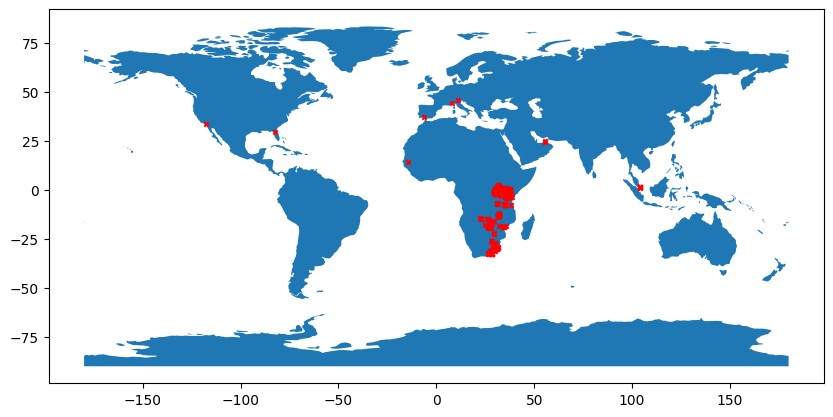
\includegraphics[scale=0.25]{before_outlier_remove.png}&
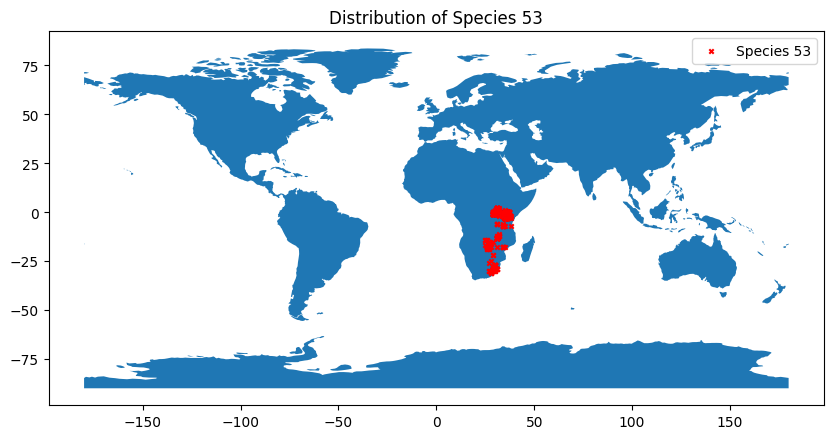
\includegraphics[scale=0.25]{After_Outlier_Removal.png}\end{tabular}
\caption{Species ID = 53 Distribution Before/After Outlier Removal (Global->Local)}
\label{Fig:Race}
\end{figure}
\section{Exploratory data analysis}
High correlation of features can lead some ML models to over weight on particular features.  In our dataset a significant number of sightings of different species are highly correlated and feature engineering may help model performance.  Over 4,836 pairs of species have a Pearson correlation co-efficient greater than 0.8 (there were no coefficients < -0.8).  This reflects that species do co-exist in common locations but it is also likely to be impacted by bias in the collection of data from common survey areas.  

Bioclimate variables (features for our modelling) also demonstrate high levels of correlation with each other.  Removing those with a Pearson correlation coefficient of more than 0.8 reduces the number of bioclimate features by half (see Figure 3) .

\begin{figure}[H]
    \centering
    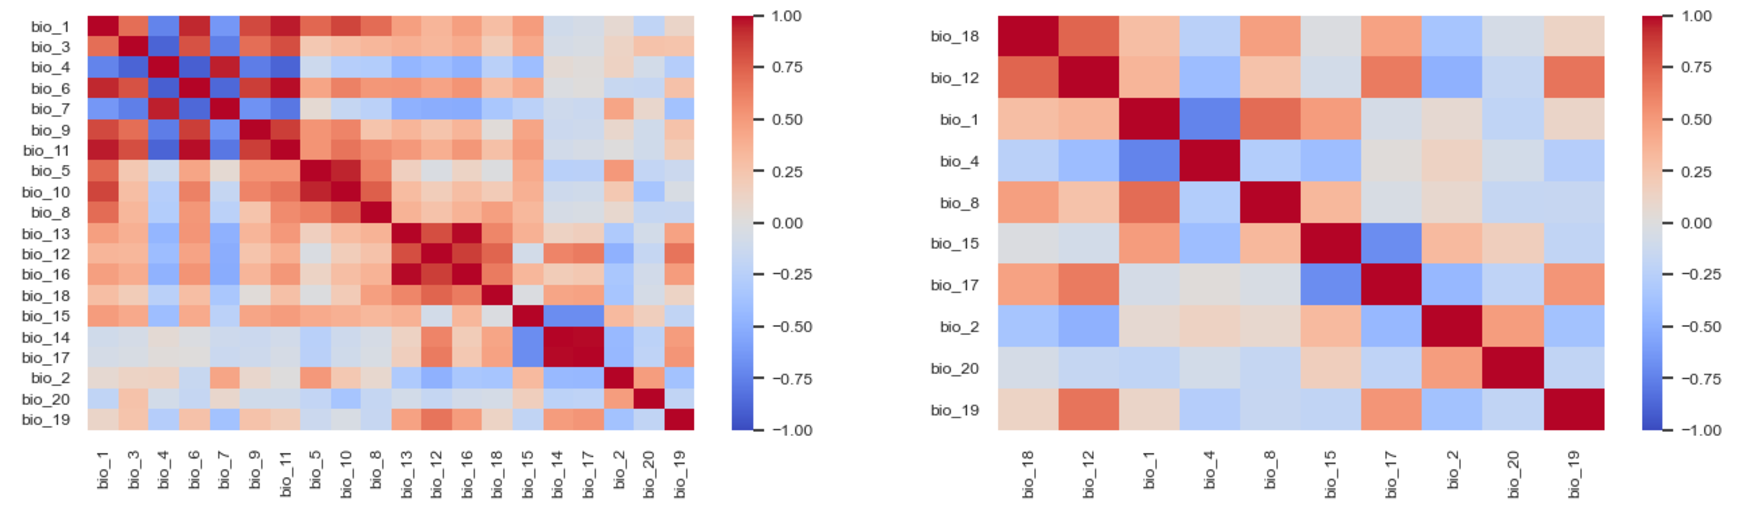
\includegraphics[width=1\linewidth]{Bio_Climate_XC.png}
    \caption{(LHS) Pearson correlation co-efficient for bioclimate data \\.\hspace{1.3cm}(RHS) Bioclimate variables removed so none coefficients > 0.8}
    \label{fig:Pearson correlation}
\end{figure}
To assess in more detail the importance and principal components of the spatial and bioclimatic features we have undertaken Principal Component Analysis (PCA). First, we standardize features and reduce the impact of outliers by limiting extreme values to a predefined range, thus enhancing the robustness of the PCA results. The eigenvectors (principal components) represent the directions of max variance in the data, and feature importance provided insight into the dominant factors.   The elbow plot shows the first 6 principal components (PCs) account for 95\% of the variance and hence we have used these 6 PCs in the model runs where PCA is applied. 

This analysis demonstrates the core variables that require emphasis in modelling species' spatial and environmental interactions. By understanding these key factors, researchers can focus on high-impact variables for further ecological studies or policy-making.

\begin{figure}[H]
    \centering
    \begin{subfigure}[b]{0.48\linewidth}  % Adjust width for each image
        \centering
        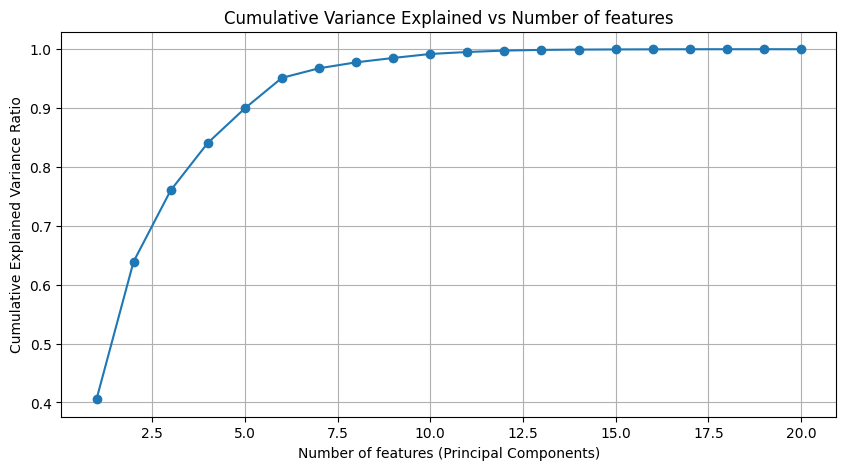
\includegraphics[width=\linewidth]{Cumulative Variance Explained vs Number of features.png}
        \caption{}
    \end{subfigure}
    % \hspace{0.1cm}  % Space between images
    \begin{subfigure}[b]{0.48\linewidth}
        \centering
        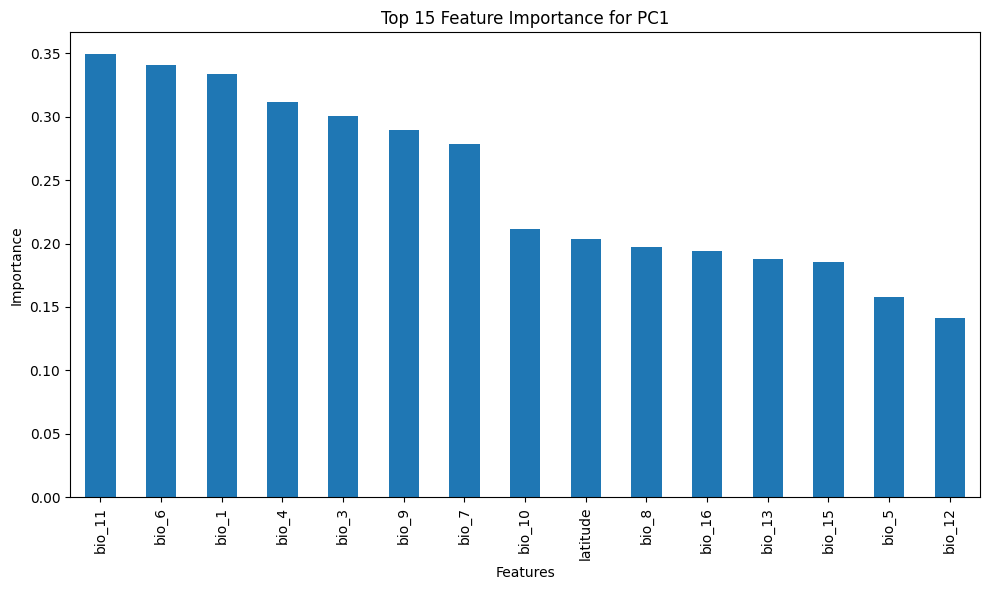
\includegraphics[width=\linewidth]{Feature Importance for id = 53.png}
        \caption{}
    \end{subfigure}
    \hspace{0.1cm}
    \caption{(a) Elbow plot of cumulative variance vs Principal Components used.  (b) Feature importance}
\end{figure}

\section{Learning methods}

\begin{table}[H]
    \centering
    \begin{tabular}{|c|c|}
\hline 
 Model& Why Chosen\\ \hline 
%  Naive Bayes& Quick to train and predict

% \\&Useful for comparing performance of more complex models
% \\&Easy to understand the model's decision-making process\\ \hline 
         Random Forest&  Less prone to overfitting, handles imbalanced data well

\\&Can handle both numerical and categorical features

\\&Performs well with large numbers of features

\\&Provides insights into the relative importance of features

\\&Can handle missing values and perform some feature selection\\ \hline 
         XGBoost&  Efficient and accurate
\\&Regularization to prevent overfitting
\\&Handles imbalanced and correlated data\\ \hline 
         SVM &  Effective in high-dimensional spaces
\\&Strong theoretical foundation and good generalization performance
\\&Handles imbalanced data through class weighting\\&Kernel trick for non-linear decision boundaries\\ \hline 
         MaxEnt &  Specifically designed for species distribution modeling
\\&Accounts for presence-only data\\&Provides insights into the importance of environmental variables
\\&Flexible to incorporate different types of environmental data\\ \hline
    \end{tabular}
    \caption{Reasons for Choosing Model}
    \label{tab:Reasons for Choosing Model}
\end{table}

% \textbf{Naive Bayes} - Explain why chosen\\
% Naive Bayes is often used as a baseline for classification problems due to its simplicity and speed. It is based on the Bayes Theorem and assumes feature importance. This assumption even though it makes modelling computationally efficient is why it cannot be used in this scenario. The features used, both bio climatic variables and species location, are known to be inter-dependant. This makes it unsuitable for actual classification but it provides a baseline to measure further models on.

% \begin{itemize}
%     \item baseline for ML methods
%     \item significant concerns due to imbalanced data and iid requirement
%     \item explain hyper-parameters and tuning
% \end{itemize}
\textbf{Random Forest (RF):} RF is an ensemble learning algorithm used for classification and regression tasks. It combines multiple decision tress. RF is less prone to overfitting and works well with high dimensional data. Moreover, it does not require major preprocessing like normalising and removal of correlated features. However, training the model can be computationally expensive and resource intensive. In previous SDM work RFs have performed well even with imbalanced or correlated data.\\
% \begin{itemize}
%     \item Referenced in literature
%     \item able to handle imbalanced data
%     \item good wit correlated data
%     \item Usually better without PCA (can mask non-linear relationships and reduces interpretability)
%     \item explain hyper-parameters and tuning
% \end{itemize}
\textbf{XGBoost (XGB):} XGB is an advanced implementation of gradient boosting, a technique that builds a model incrementally by training each new model to correct the errors of the previous model.  XGBoost uses a series of decision trees where each new tree aims to reduce the errors of the previous tree. A major improvement of XGB over other gradient boosters is its inclusion of regularization to prevent overfitting. The algorithm also works well with imbalanced and correlated data. PCA is not necessary for XGB however it can be usefule to compare results.\\

Unlike random forest where the tress are built in parallel the trees are built sequentially. While this might be computationally easier it does increase training times as the size of the dataset and the number of trees increases. Another drawback of XGBoost is that it can be less interpretable \\

% \begin{itemize}
%     \item Referenced in literature
%     \item able to handle imbalanced data
%     \item good wit correlated data
%     \item   PCA not necessary but worth comparing (can mask non-linear relationships and reduces 
%     \item explain hyper-parameters and tuninginterpretability)
% \end{itemize}
\textbf{Support Vector Machine (SVM)}: SVM is a powerful supervised machine learning algorithm used primarily for classification tasks. SVM aims to find the best possible boundary (called a hyperplane) that separates data points into different classes. This boundary is chosen to maximize the margin between the classes.  SVM can handle correlated features and high-dimensional spaces like our data. It can also handle imbalanced data through the use of class weights, allowing for penalization of misclassification of the minority class.  However it has high training times forcing the hyperparameter space to be smaller to improve efficiency. 

% A few key hyper parameters considered while modelling:\\
% The function to map the original data to a higher-dimensional space where a linear hyperplane can be used for separation. - kernel\\
% Parameter to control the trade-off between maximizing the margin and minimizing classification error. - C\\
% Controls the influence of higher-degree polynomials and the sigmoid function - Coef0\\
% Parameter that defines the influence of a single training example - gamma\\

% Class Weight (class_weight): Helps in dealing with imbalanced data by adjusting the weight given to each class.
% \begin{itemize}
%     \item     Referenced in literature
%     \item able to handle imbalanced data
%     \item good with correlated data
%     \item   PCA not necessary but worth comparing (can mask non-linear relationships and reduces 
%     \item explain hyper-parameters and tuning
% \end{itemize}
\textbf{MaxEnt}: MaxEnt is a machine learning method often applied to SDM and is considered one of the benchmarks for modelling presence only data. The purpose is to maximise the distribution of possible data (entropy), making the model as uniform and unbiased as it can while still being able to fit to the input data. MaxEnt measures the probability distribution of different species across a geographical area using environmental variables and presence only occurrences, which is useful for our task.

MaxEnt models species distribution based on environmental variables and background points. The background points are introduced to represent pseudo-absence data\cite{pseudo-absences}. MaxEnt has only a few hyperparameters, we found the optimum number of background points to be 10,000, This ensured we captured the environmental conditions, but limited the risk of overfitting.  We set iterations to 500 so the model converged but not to computational inefficiency. We used 5 fold cross validation consistent with the other models. 

MaxEnt has a defined structure for input and output data so there were differences in data prep and outputs to our other models.  We used binned occurrence data for the target species.  MaxEnt  uses continuous environmental data for features No other species data was used. We removed the highly correlated bioclimate data (shown in the analysis above) as MaxEnt is poor at handling correlated input data.  We did not use PCA as we wanted to maintain interpretability of the climate feature importance.   We used the area under an ROC curve to compare to other models as P-R data was not available from our version of MaxEnt.

\section{Results}

Models were evaluated on normalised data using 5 fold cross validation to compare performance.  This ensured that each model gave consistent results. The 3 models (RF, XGBoost and SVM) were run on the different approaches to data preparation.  PR AUC values were used to select the best model and data preparation process . PR AUC was used over ROC AUC or other metrics because the data available is highly imbalanced towards the negative side and, in such cases, PR AUC provides a better measure of model performance.

15 target species were randomly selected from species with the highest spatial distributions ( top decile number of bins) to optimize the models. The target species was set as the variable to be predicted while all the other species served as features. This was then repeated over 15 different target species along with hyperparameter tuning to get the optimal set of hyperparameters. These were then generalised to all the other species in the data. The newly obtained hyperparameters were tested over a set of 10 different species to evaluate whether they perform accordingly. 

The models were initially run over the training data in its raw form (post data quality and binning) to baseline the performance of each model (fig 5.a). Random Forest and XGBoost gave PR AUC values of 0.773 and 0.742 while SVM performed poorly. Better results were achieved by fine tuning hyperparameters and by training models on regional data. The maximum PR AUC score of 0.786 was achieved by running Random Forest over a variation of the data containing the species in a region and the principal components of the environmental data accounting for 95\% of the variation(fig 5.f). The next best score of 0.775 was from the Random Forest model using all global data with fine tuned hyperparameters(fig 5.b). Even though this is a good score training with the global data over all the species becomes computationally expensive and time consuming.

The MaxEnt algorithm achieved an average ROC AUC score of 0.9503 by running over the different target species. This score though good is still outperformed by Random Forest and XGBoost running on the global data with tuned hyperparameters.
\begin{figure}[H]
    \centering
    \begin{subfigure}[b]{0.15\linewidth}  % Adjust width for each image
        \centering
        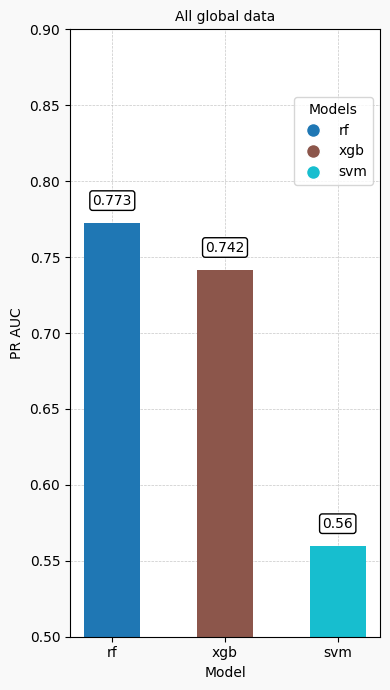
\includegraphics[width=\linewidth]{All global data.png}
        \caption{}
        \label{fig:global_data}
    \end{subfigure}
    \hspace{0.1cm}  % Space between images
    \begin{subfigure}[b]{0.15\linewidth}
        \centering
        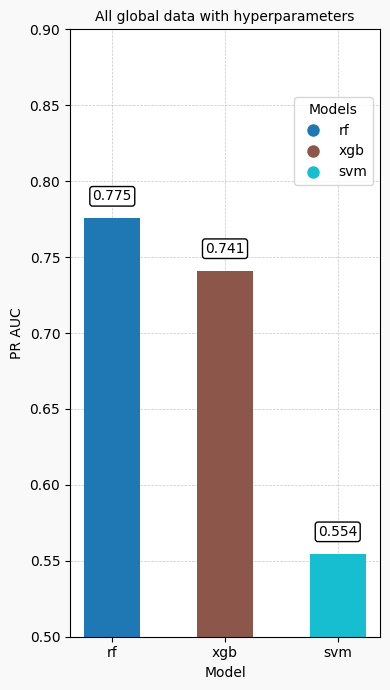
\includegraphics[width=\linewidth]{All global data with hyperparameters.png}
        \caption{}
        \label{fig:global_data_hyperparams}
    \end{subfigure}
    \hspace{0.1cm}
    \begin{subfigure}[b]{0.15\linewidth}
        \centering
        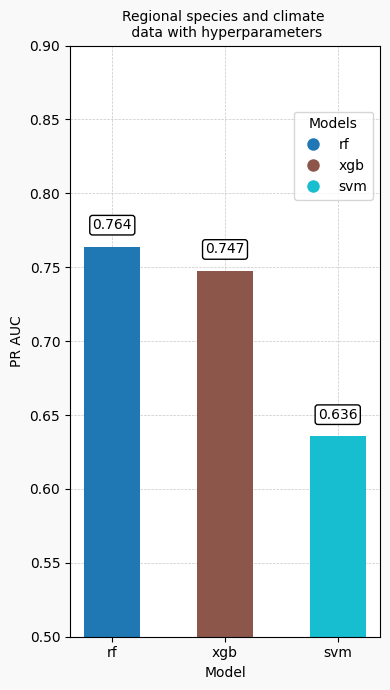
\includegraphics[width=\linewidth]{Regional species and climate data with hyperparameters.png}
        \caption{}
        \label{fig:regional_species_climate}
    \end{subfigure}
    \hspace{0.1cm}
    \begin{subfigure}[b]{0.15\linewidth}
        \centering
        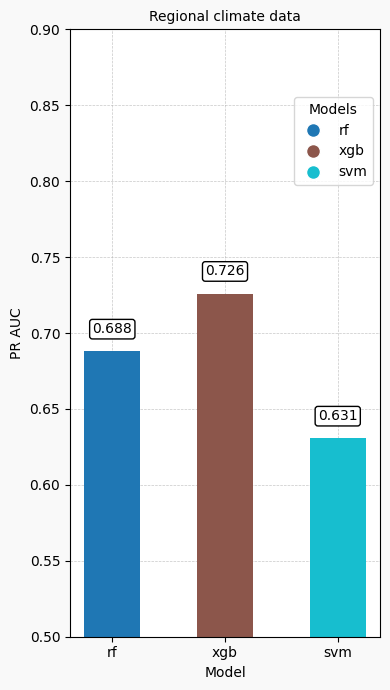
\includegraphics[width=\linewidth]{Regional climate data'.png}
        \caption{}
        \label{fig:regional_climate}
    \end{subfigure}
    \hspace{0.1cm}
    \begin{subfigure}[b]{0.15\linewidth}
        \centering
        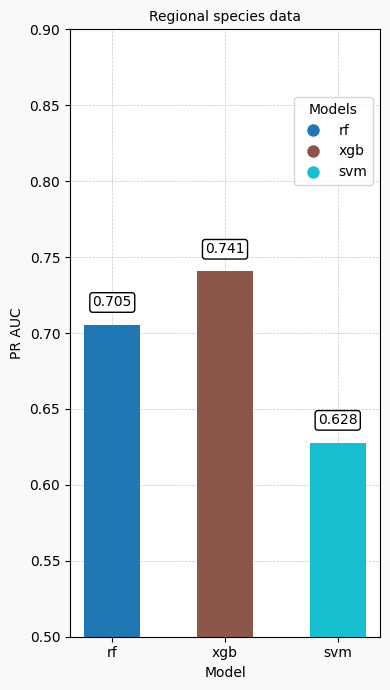
\includegraphics[width=\linewidth]{Regional species data.png}
        \caption{}
        \label{fig:regional_species}
    \end{subfigure}
    \hspace{0.1cm}
    \begin{subfigure}[b]{0.15\linewidth}
        \centering
        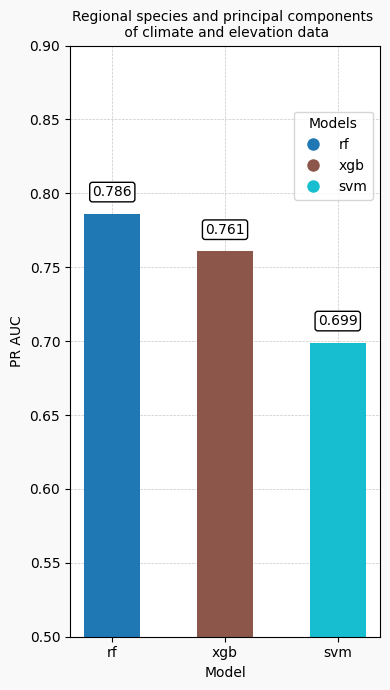
\includegraphics[width=\linewidth]{Regional species and principal components of climate and elevation data.png}
        \caption{}
        \label{fig:regional_species_pca}
    \end{subfigure}
    \caption{Comparing the PR AUC of the models over different variations of data.}
    \label{fig:all_images_side_by_side}
\end{figure}
\begin{table}[H]
    \centering
    \begin{tabular}{|c|c|}
\hline 
 Scenario No.& Input data (All data has outliers removed)\\ \hline 
Scenario 1 & Global species and climate data without hyperparameter tuning\\ \hline
Scenario 2 & Global species and climate data\\ \hline
Scenario 3 & Regional species and climate data\\ \hline
Scenario 4 & Regional climate data\\ \hline
Scenario 5 & Regional species data\\ \hline
Scenario 6 & Regional species data and principal components of climate data\\ \hline
    \end{tabular}
    \caption{Different scenarios of data preprocessing}
    \label{tab:Different scenarios of model runs}
\end{table}
\section{Inferences}
Both Random Forest and XGBoost performed well over all variations, in most cases with Random Forest coming up on top. SVM however performs poorly, this could be due to the imbalance of the data as the algorithm performs noticeable better on regional datasets with the less sparse values. The best values were with Random Forest running on the principal components of the environmental species and the species data, but this brings up the problem of feature interpretability being harder. 

Though the models seem to work well with the global data this might not be the most optimal solution as trying to make predictions for each species on a global scale would make modelling computationally expensive and time consuming. Moreover the additional data from regions remote to the species taken as the target, logically should not be of importance to the model.

The MaxEnt model, though it run almost as well the best performing model, is not viable here as it is time consuming to run and it requires more complex tuning and preprocessing. 

The MaxEnt model though it was mentioned extensively in the literature did not perform as well as the Random Forest algorithm. This could be because of the data being extremely imbalanced or because of the non linear relationships between the features which could not be addressed properly 

\section{Conclusions}

Overall the best combination after assessing computational availability, different ML models and different approaches data preparation was  to use Random Forest on the principal components of the bio climate data plus the other species data as features .

The models choosen were based on their ability to handle the challenges of the dataset provided and RF and XGBoost demonstrated good performance, SVM to a lesser extent.  Notably, RF and XGB performed well without us specifically adding pseudo-absence data.

There are many areas we'd like to build on this work including introducing pseudo-absence data, a deeper analysis on bin sizes, and additional environmental features.  

\newpage
\section{Citations and References}
\bibliography{refs.bib}
\bibliographystyle{plain}

\section{Appendix}


\subsection{PR AUC vs ROC AUC}
PR AUC: PR AUC refers to the area under the PR curve of a model. It is a comprehensive view of the model's ability to balance precision and recall over an entire range of thresholds. It focuses more on the positive class and evaluates the trade-off between the precision and the recall. It is more sensitive to class imbalance and is often used when the cost of false positives and false negatives are significant. It is heavily influenced by how the model performs on the minority class.

ROC AUC:  ROC (Receiver Operating Characteristic) Area Under the Curve is the are under an ROC curve. It provides an overall performance of a model across all classification thresholds. The curve is a plot between the true positive rate against the false positive rate at various threshold settings. A higher ROC AUC indicates that the model is able to distinguish between positive and negative instances with a higher chance of success.

PR AUC and ROC AUC are evaluation metrics both suited for evaluating a model but the heavy imbalance of the data makes PR AUC a better option. ROC AUC will give a higher score when the data is heavily imbalanced towards one side, even if the model is not performing up to the mark. This is why PR AUC has been used as the evaluation metric during hyperparameter tuning and model comparison.

\newpage
\subsection{Hyper-parameters tuned for each ML model}


% \begin{table}
%     \centering
%     \begin{tabular}{c c}
%     ML model& Tuned hyper-parameters \\
%     Random Forest & the number of trees - n\_estimators;  maximum depth of each tree - max\_depth;
%     minimum samples required to split a node - min\_samples\_split; 
% minimum samples required to become a leaf node - min\_samples\_leaf;
% number of features considered when looking for the best split - max\_features.\\
%          XGBoost& The number of boosting rounds or trees to build - n\_estimators
% Controls the contribution of each tree to the final prediction - learning\_rate
% Maximum depth of each individual decision tree. Larger depths allow trees to model more complex relationships, but they can lead to overfitting. - max\_depth
% The minimum size of each leaf node - min\_child\_weight
% Fraction of the training data to randomly sample for each tree - subsample
% Controls whether to split a node -gamma
% Controls the balance of positive and negative weights, useful for imbalanced classes. - scale\_pos\_weight\\
%          SVM& The function to map the original data to a higher-dimensional space where a linear hyperplane can be used for separation. - kernel
% Parameter to control the trade-off between maximizing the margin and minimizing classification error. - C
% Controls the influence of higher-degree polynomials and the sigmoid function - Coef0
% Parameter that defines the influence of a single training example - gamma\\
%          & \\
%     \end{tabular}
%     \caption{Caption}
%     \label{tab:my_label}
% \end{table}

\begin{table}[h!]
    \centering
    \resizebox{\textwidth}{!}{
    \begin{tabular}{|c|l|}
    \hline
    \textbf{ML Model} & \textbf{Tuned Hyper-parameters} \\
    \hline
    \multirow{5}{*}{Random Forest} 
    & \textbf{n\_estimators}: the number of trees \\
    & \textbf{max\_depth}: maximum depth of each tree \\
    & \textbf{min\_samples\_split}: minimum samples required to split a node \\
    & \textbf{min\_samples\_leaf}: minimum samples required to become a leaf node \\
    & \textbf{max\_features}: number of features considered when looking for the best split \\
    \hline
    \multirow{6}{*}{XGBoost} 
    & \textbf{n\_estimators}: number of boosting rounds or trees to build \\
    & \textbf{learning\_rate}: controls the contribution of each tree to the final prediction \\
    & \textbf{max\_depth}: maximum depth of each individual decision tree \\
    & \textbf{min\_child\_weight}: minimum size of each leaf node \\
    & \textbf{subsample}: fraction of the training data to randomly sample for each tree \\
    & \textbf{gamma}: controls whether to split a node \\
    & \textbf{scale\_pos\_weight}: controls the balance of positive and negative weights (useful for imbalanced classes) \\
    \hline
    \multirow{4}{*}{SVM} 
    & \textbf{kernel}: function to map the original data to a higher-dimensional space for separation \\
    & \textbf{C}: controls the trade-off between maximizing the margin and minimizing classification error \\
    & \textbf{Coef0}: controls the influence of higher-degree polynomials and the sigmoid function \\
    & \textbf{gamma}: defines the influence of a single training example \\
    \hline
    \end{tabular}
    }
    \caption{Tuned Hyper-parameters for ML Models}
    \label{tab:my_label}
\end{table}


\subsection{Pearson's Cross Correlation of Species Data (500 species)}
Clustered heatmap of Pearson's cross correlation between 500 species showing significant number of groups of highly correlation.
\begin{figure}
    \centering
    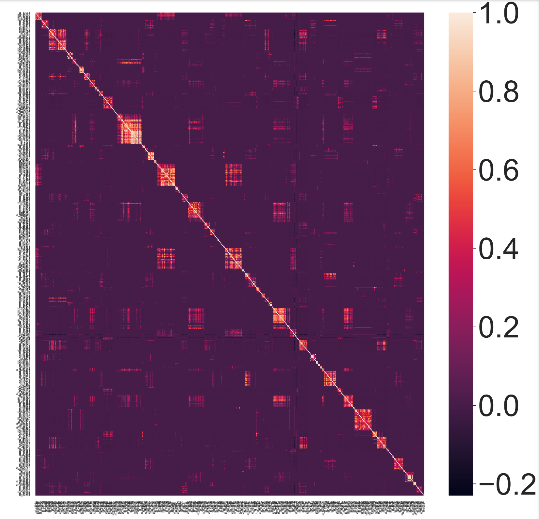
\includegraphics[width=1\linewidth]{Species_Cross_Correlation.png}
    \caption{Clustered Pearson's Cross Correlation of Species Data (500 species)}
    \label{fig:enter-label}
\end{figure}

\clearpage

\end{document}

%%% Local Variables:
%%% mode: latex
%%% TeX-master: t
%%% End:


